\begin{figure}[hbt]
    \centering
    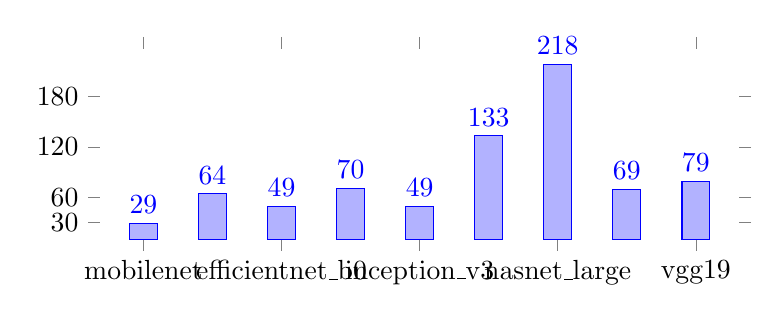
\begin{tikzpicture}
      \begin{axis}[ybar,
            width=100mm, height=40mm,
            x axis line style = { opacity = 0 },
            symbolic x coords = {mobilenet, nasnet\_mobile, efficientnet\_b0, xception, inception\_v3, efficientnet\_b5, nasnet\_large, vgg16, vgg19},
            ytick={30,60,120,180,240},
            nodes near coords,
        ]
        \addplot coordinates { 
            (mobilenet,         29)
            (nasnet\_mobile,    64)
            (efficientnet\_b0,  49)
            (xception,          70)
            (inception\_v3,     49)
            (efficientnet\_b5, 133)
            (nasnet\_large,    218)
            (vgg16,             69)
            (vgg19,             79)
        };
      \end{axis}
    \end{tikzpicture}
    
    \caption{Figure: Average Training Time in seconds}
    \label{img:avg-train-time}


    \vspace{2mm}
    Workstation: Ryzen 2700x (8/16 Cores), 16Gb RAM, GTX 1060 6Gb, TensorFlow Compute Capability: 6.1
\end{figure}


